\chapter{Protocol of work so far}
\section{Rotated lines experiment}

\subsection{Introduction}
The goal of this task was to recreate example 2 from \citet{nessler}. In this example they fed a winner-take-all spiking neural network images with lines in different orientations on them. The network then clustered the images into ten groups depending on their orientation.

\subsection{Methods}
\paragraph{Input data}
The images used in this task were generated with a size of 29 x 29 pixel. Black lines going through the center of the image were drawn onto a white background. To simulate noise each pixel had a ten percent chance to have its color flipped. To ensure that all lines in the images have the same length regardless of their orientation a circular mask with a radius of 15 pixel was applied to the images. This recolored all pixel outside of the mask to white. During the training of the network these images were generated in uniformly distributed orientations for each training step. The random chosen orientation could lie between 0 and 359 degrees.  Two examples of such images can be seen in figure \ref{fig:angleImages}.

\begin{figure}
  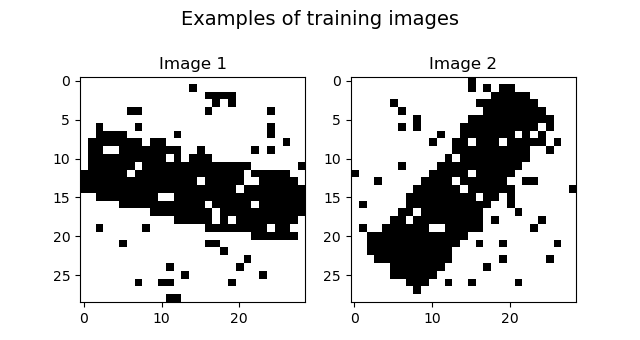
\includegraphics[width=\linewidth]{figures/angleNetwork/trainingImages.png}
  \caption{Two examples of the generated training data in this experiment.}
  \label{fig:angleImages}
\end{figure}

\paragraph{Neuron model}

\paragraph{Network architecture}
Each pixel of an input image was connected to two neurons. The first of these neurons is in an active state when the pixel is black and in an inactive state otherwise. The second neuron expresses the opposite behaviour. As a consequence the network needs 1682 ($29 \cdot 29 \cdot 2$) excitatory input neurons $x_1,...,x_n$. These X neurons are then fully connected to ten excitatory output neurons $y_1,...,y_k$. The Y neurons are modelled in a winner-takes-all (WTA) circuit. This means that whenever one Y neuron spikes, an inhibitory signal is fed to all Y neurons, thus preventing the further activation of all output neurons for 5 ms. After training each Y neuron should be active for lines in an 18° area. 


\paragraph{Inhibition}
The inhibition signal depends on the current membrane potential of the Y neurons.


\begin{equation}
\label{eqn:iinh}
I(t) = \begin{dcases*} \ln ( \sum_{i=1}^k e^{U_k} ) & if any $y(t^f) = 1$, i.e. any y fired in $ [t^f - \sigma, t^f] $ \\
0 & \text{if any $ y(t^f) = 0 $, i.e. any y did not fire in $ [t^f - \sigma, t^f] $ } \end{dcases*}\end{equation}




Excitatory input:
The intrinsic weights of the x neurons were omitted in this experiment. This was chosen because there was no benefit in including them.
\begin{equation}
\label{eqn:uk}
U_k(t) = \sum_{i=1}^n w_{ki} \cdot x_i(t)
\end{equation}

Firing rate:
\begin{equation}
\label{eqn:rk}
r_k(t) = e^{u_k(t) - I(t)}
\end{equation}

Chance to spike within time step $\delta t$:
\begin{equation}
\label{eqn:rkdt}
r_k(t) \cdot \delta t
\end{equation}

Weight updates:
\begin{equation}
\label{deltawki}
\Delta w_{ki} = \begin{dcases*} ce^{-w_{ki}} - 1 & if $x_{i}(t^f) = 1$, i.e.$x_{i}$ fired in $ [t^f - \sigma, t^f] $ \\
-1 & \text{if $ x_i(t^f) = 0 $, i.e. $ x_i $ did not fire in $ [t^f - \sigma, t^f] $ } \end{dcases*}
\end{equation}

\subsection{Results}
